% Requires: \usepackage{tikz,float,xcolor}  \usetikzlibrary{arrows.meta,positioning,calc}
% Compile with pdflatex (or xelatex/lualatex for direct UTF-8 accents).
\documentclass[tikz,border=10pt]{standalone}
\usepackage[utf8]{inputenc}
\usepackage[T1]{fontenc}
\usepackage{float}
\usepackage{xcolor}
\usetikzlibrary{arrows.meta,positioning,calc}

\begin{document}
\begin{figure}[H]
\centering
\small
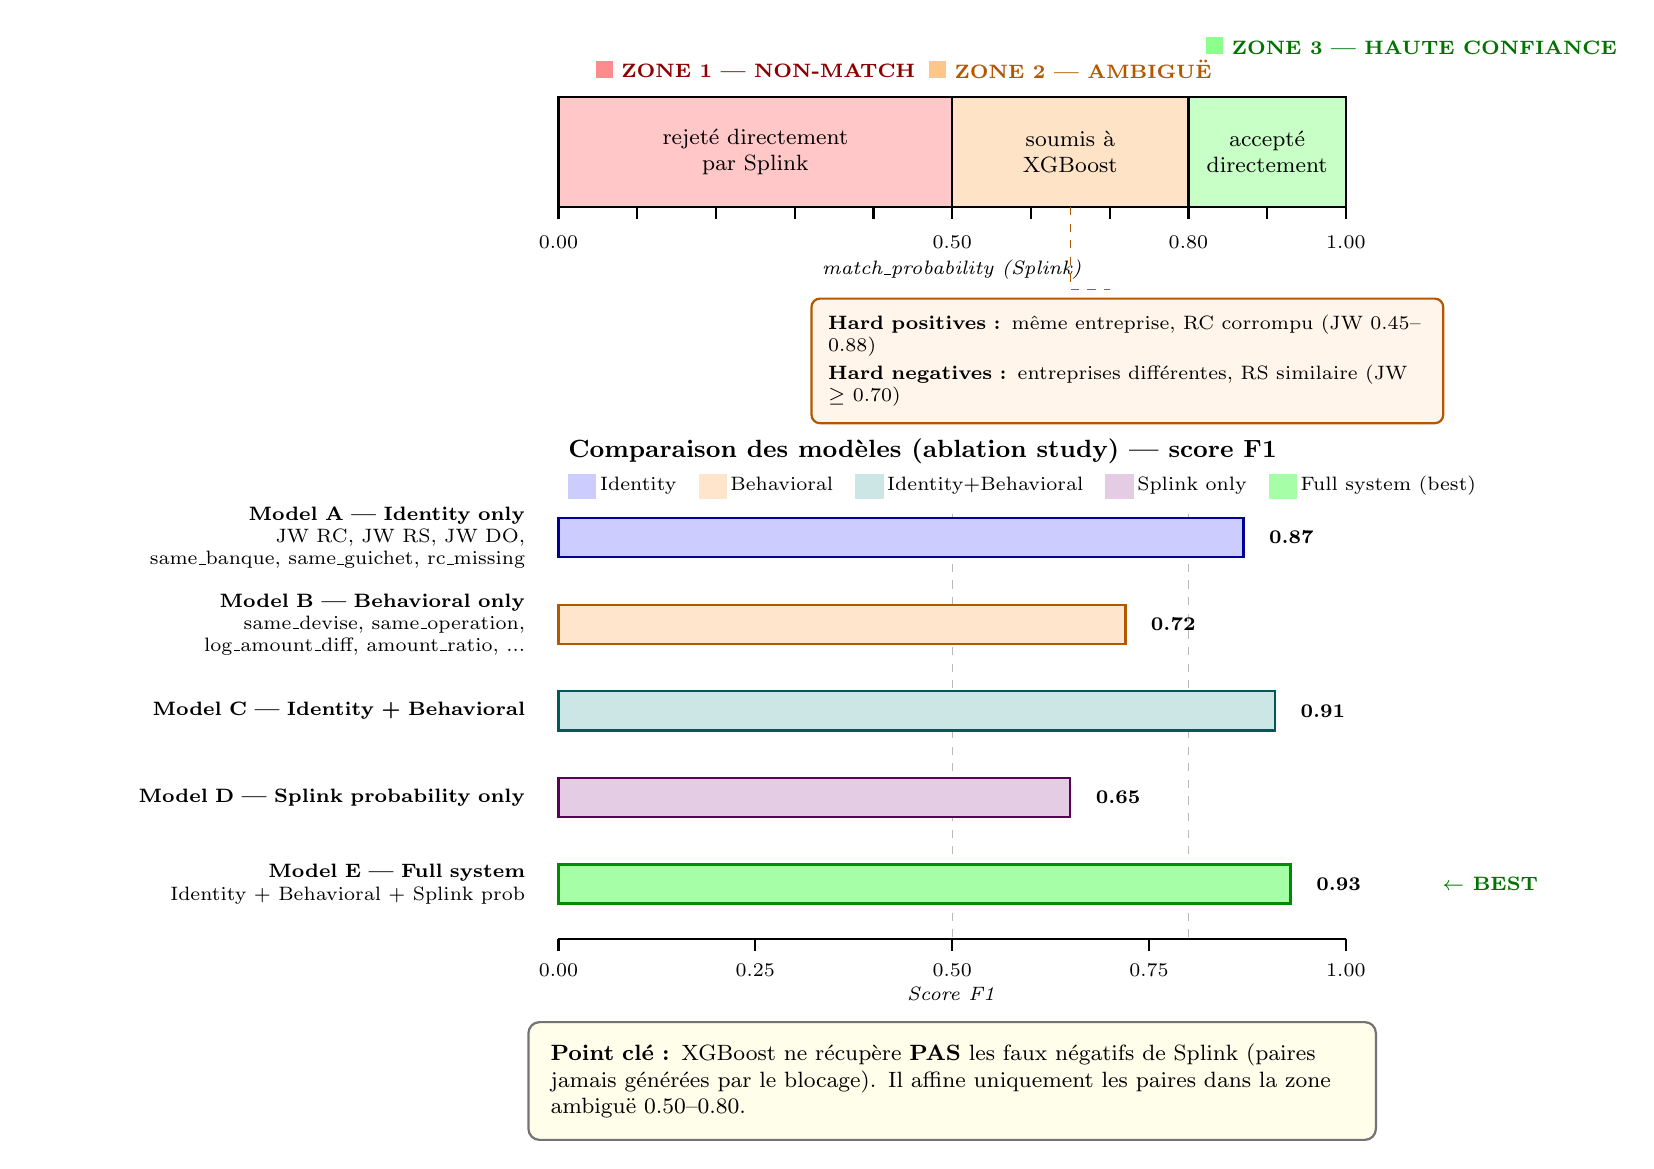
\begin{tikzpicture}[every node/.style={font=\small}]

% ======================================================================
% TOP : PROBABILITY AXIS WITH 3 CONFIDENCE ZONES  (scale: 10 units = 1.0)
% ======================================================================
\fill[red!22]    (0,0) rectangle (5,1.4);
\fill[orange!22] (5,0) rectangle (8,1.4);
\fill[green!22]  (8,0) rectangle (10,1.4);
\draw[thick] (0,0) rectangle (10,1.4);
\draw[thick] (5,0) -- (5,1.4);
\draw[thick] (8,0) -- (8,1.4);

% zone headers (above the band) + small inline tikz colour chips
\node[anchor=center, font=\bfseries\scriptsize, text=red!55!black] at (2.5,1.75)
  {\tikz{\fill[red!45] (0,0) rectangle (0.22,0.22);}\ ZONE 1 --- NON-MATCH};
\node[anchor=center, font=\bfseries\scriptsize, text=orange!70!black] at (6.5,1.75)
  {\tikz{\fill[orange!45] (0,0) rectangle (0.22,0.22);}\ ZONE 2 --- AMBIGUË};
\node[anchor=west, font=\bfseries\scriptsize, text=green!45!black] at (8.1,2.05)
  {\tikz{\fill[green!45] (0,0) rectangle (0.22,0.22);}\ ZONE 3 --- HAUTE CONFIANCE};

% subtitles inside the bands
\node[align=center, font=\footnotesize] at (2.5,0.7) {rejeté directement\\par Splink};
\node[align=center, font=\footnotesize] at (6.5,0.7) {soumis à\\XGBoost};
\node[align=center, font=\footnotesize] at (9,0.7)   {accepté\\directement};

% axis baseline ticks (y=0 is the bottom edge of the coloured band)
\foreach \x in {0,1,2,3,4,5,6,7,8,9,10}{
  \draw[thick] (\x,0) -- (\x,-0.15);
}
\node[font=\scriptsize] at (0,-0.45)  {0.00};
\node[font=\scriptsize] at (5,-0.45)  {0.50};
\node[font=\scriptsize] at (8,-0.45)  {0.80};
\node[font=\scriptsize] at (10,-0.45) {1.00};
\node[font=\scriptsize] at (5,-0.8) {\textit{match\_probability (Splink)}};

% connector + callout for the ambiguous-zone annotation
\draw[dashed, orange!70!black] (6.5,0) -- (6.5,-1.05) -- (7,-1.05);
\node[rectangle, rounded corners=3pt, draw=orange!70!black, thick, fill=orange!8,
      font=\scriptsize, align=left, text width=7.6cm, inner sep=6pt,
      anchor=north west] (callout) at (3.2,-1.15)
  {\textbf{Hard positives :} même entreprise, RC corrompu (JW 0.45--0.88)\\[2pt]
   \textbf{Hard negatives :} entreprises différentes, RS similaire (JW $\geq$ 0.70)};

% ======================================================================
% MIDDLE : 5-MODEL ABLATION COMPARISON (F1 score, same 0--1 scale)
% ======================================================================
\node[font=\bfseries\small, anchor=west] at (0,-3.1)
  {Comparaison des modèles (ablation study) --- score F1};

\node[font=\scriptsize, anchor=west] at (0,-3.55)
  {\colorbox{blue!20}{\phantom{x}}\,Identity\quad
   \colorbox{orange!20}{\phantom{x}}\,Behavioral\quad
   \colorbox{teal!20}{\phantom{x}}\,Identity+Behavioral\quad
   \colorbox{violet!20}{\phantom{x}}\,Splink only\quad
   \colorbox{green!35}{\phantom{x}}\,Full system (best)};

% vertical guide lines tying back to the 0.50 / 0.80 thresholds above
\draw[dashed, gray!55] (5,-3.9) -- (5,-9.3);
\draw[dashed, gray!55] (8,-3.9) -- (8,-9.3);

% ---- Model A : Identity only ----
\node[anchor=east, align=right, font=\scriptsize, text width=6.2cm] at (-0.3,-4.2)
  {\textbf{Model A --- Identity only}\\
   JW RC, JW RS, JW DO, same\_banque, same\_guichet, rc\_missing};
\fill[blue!20, draw=blue!60!black, thick] (0,-4.45) rectangle (8.7,-3.95);
\node[anchor=west, font=\scriptsize\bfseries] at (8.9,-4.2) {0.87};

% ---- Model B : Behavioral only ----
\node[anchor=east, align=right, font=\scriptsize, text width=6.2cm] at (-0.3,-5.3)
  {\textbf{Model B --- Behavioral only}\\
   same\_devise, same\_operation, log\_amount\_diff, amount\_ratio, ...};
\fill[orange!20, draw=orange!70!black, thick] (0,-5.55) rectangle (7.2,-5.05);
\node[anchor=west, font=\scriptsize\bfseries] at (7.4,-5.3) {0.72};

% ---- Model C : Identity + Behavioral ----
\node[anchor=east, align=right, font=\scriptsize, text width=6.2cm] at (-0.3,-6.4)
  {\textbf{Model C --- Identity + Behavioral}};
\fill[teal!20, draw=teal!70!black, thick] (0,-6.65) rectangle (9.1,-6.15);
\node[anchor=west, font=\scriptsize\bfseries] at (9.3,-6.4) {0.91};

% ---- Model D : Splink probability only ----
\node[anchor=east, align=right, font=\scriptsize, text width=6.2cm] at (-0.3,-7.5)
  {\textbf{Model D --- Splink probability only}};
\fill[violet!20, draw=violet!70!black, thick] (0,-7.75) rectangle (6.5,-7.25);
\node[anchor=west, font=\scriptsize\bfseries] at (6.7,-7.5) {0.65};

% ---- Model E : Full system (BEST) ----
\node[anchor=east, align=right, font=\scriptsize, text width=6.2cm] at (-0.3,-8.6)
  {\textbf{Model E --- Full system}\\
   Identity + Behavioral + Splink prob};
\fill[green!35, draw=green!55!black, very thick] (0,-8.85) rectangle (9.3,-8.35);
\node[anchor=west, font=\scriptsize\bfseries] at (9.5,-8.6) {0.93};
\node[anchor=west, font=\bfseries\scriptsize, text=green!45!black] at (11.1,-8.6) {$\leftarrow$ BEST};

% F1 axis
\draw[thick] (0,-9.3) -- (10,-9.3);
\foreach \x/\lab in {0/0.00,2.5/0.25,5/0.50,7.5/0.75,10/1.00}{
  \draw[thick] (\x,-9.3) -- (\x,-9.45);
  \node[font=\scriptsize] at (\x,-9.7) {\lab};
}
\node[font=\scriptsize] at (5,-10.0) {\textit{Score F1}};

% ======================================================================
% KEY INSIGHT BOX
% ======================================================================
\node[rectangle, rounded corners=4pt, draw=black!55, thick, fill=yellow!8,
      font=\footnotesize, align=left, text width=10.2cm, inner sep=8pt] at (5,-11.1)
  {\textbf{Point clé :} XGBoost ne récupère \textbf{PAS} les faux négatifs de Splink
   (paires jamais générées par le blocage). Il affine uniquement les paires
   dans la zone ambiguë 0.50--0.80.};

\end{tikzpicture}
\caption{Architecture de confiance à trois zones du complément XGBoost à Splink
  (\texttt{xgboost\_complement.py}).}
\label{fig:xgb-zones}
\end{figure}
\end{document}
